% ============================================================
% Week 5 -- Estimation, inference and assessment in simple linear regression
% ============================================================
\chapter{Inference for Linear Models and Computation in R}\label{ch:week05}

This chapter covers Week~5 (Lectures 15--18). \textbf{Source caveat.} The instructor's Week-5 lecture notes
(\texttt{Feb21.pdf}) were \emph{not} accessed. The chapter is built from the Week-5 R code (\texttt{Feb21.r}), the
Week-5 assignment (\texttt{hw56.pdf}), and the standard theory that the code and assignment use. The theory is written
in the notation of the earlier chapters. Every numerical value shown was reproduced in the companion notebooks.

% ============================================================
% Lecture 15 -- Estimating the coefficients of linear models
% ============================================================
\section{Estimating the Coefficients of Linear Models}\label{sec:L15}

\lectureheader{15}{qF9VBw3CP78}{Week-5 R code \texttt{Feb21.r} (least squares fit of \texttt{iris}, normal equations by hand) and Week-5 assignment Q4. The Week-5 lecture PDF was \emph{not} accessed. The derivations below follow the titles and code and are marked accordingly.}

\begin{guiding*}
By the end of this lecture you should be able to:
\begin{itemize}
  \item compute $\hat\beta=(X\T X)^{-1}X\T Y$ for a full-rank model, by hand and in code;
  \item prove that $\hat\beta$ is unbiased with $\Cov(\hat\beta)=\sigma^2(X\T X)^{-1}$;
  \item derive $\Var(\hat\beta_0)$, $\Var(\hat\beta_1)$ and $\Cov(\hat\beta_0,\hat\beta_1)$ in simple linear regression;
  \item fit and plot a regression line with \texttt{lm}/\texttt{statsmodels}.
\end{itemize}
\end{guiding*}

\subsection{Recap}
Week~4 established that least squares estimates are the solutions of the normal equations
$X\T X\beta=X\T Y$ (\cref{thm:L12-normal}). The solution is unique iff $\rank X=p$
(\cref{cor:L12-fitted}), and $X\hat\beta=\PX Y$ (\cref{prop:L14-PX}). Week~5 applies this theory to
regression models, which in practice almost always have a full-rank $X$. Throughout this chapter we
write simple linear regression as
\[
Y_i=\beta_0+\beta_1x_i+\eps_i,\qquad i=1,\dots,n,
\]
the notation of the R output (``\texttt{(Intercept)}'' and the slope). In Week~2 we called these
coefficients $a_1,a_2$.

\subsection{The iris example from the R code}
\begin{example}[Sepal length on petal width]\label{ex:L15-iris}
The R code fits \texttt{lm(Sepal.Length \textasciitilde\ Petal.Width, data = iris)} to Fisher's iris data
($n=150$ flowers), plots the points, and adds the fitted line with \texttt{abline} and with
\texttt{ggplot(...) + stat\_smooth(method = "lm")}. The estimates are
\[
\hat\beta_0=4.7776,\qquad \hat\beta_1=0.8886 .
\]
A flower whose petals are $1$\,cm wider has, on average, sepals $0.89$\,cm longer. The line
passes through $(\bar x,\bar y)=(1.1993,\,5.8433)$ (\cref{cor:L05-props}).
\end{example}

\begin{figure}[ht]
\centering
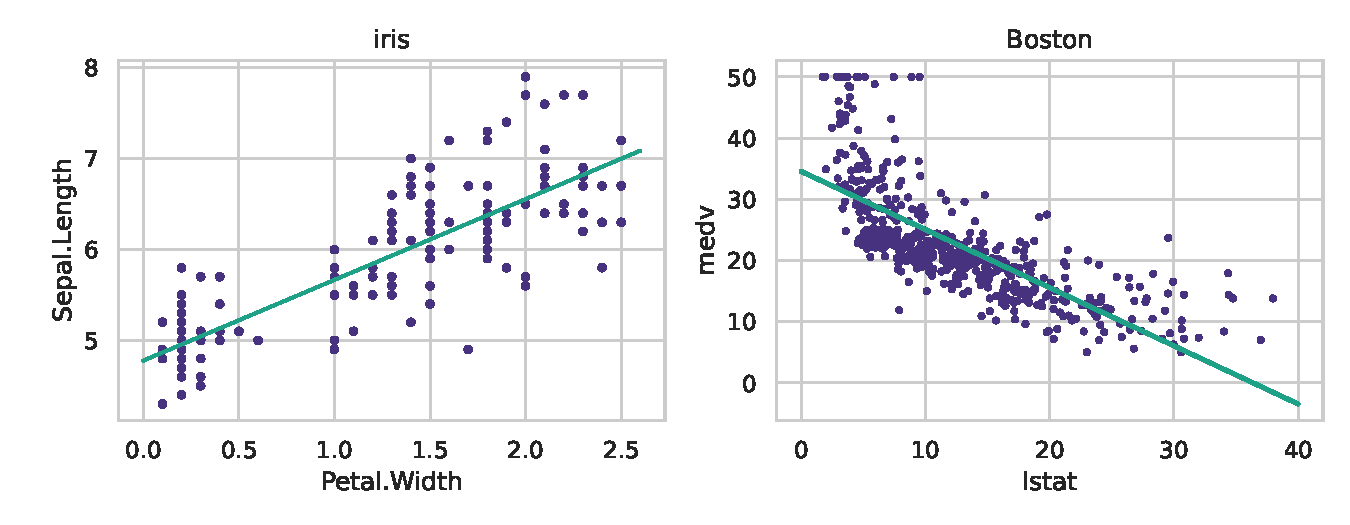
\includegraphics[width=0.95\textwidth]{figures/L15_iris_boston.pdf}
\caption{Least squares lines for \texttt{iris} (\cref{ex:L15-iris}) and for \texttt{Boston} (\cref{sec:L16}).}
\label{fig:L15-fits}
\end{figure}

\subsection{Normal equations by hand}
The second part of the R code solves the normal equations directly for a model with two
explanatory variables:
\begin{center}
\begin{minipage}{0.85\textwidth}\small\ttfamily
x1 <- c(10,0,45,56,79); x2 <- c(2,34,15,5,4)\\
y <- x1 + x2 + rnorm(5, mean=0, sd=0.3)\\
X <- as.matrix(cbind(1,x1,x2))\\
betahat = solve(t(X) \%*\% X) \%*\% (t(X) \%*\% Y) \quad \# solution of X\textasciicircum TX beta = X\textasciicircum Ty\\
lm.fit <- lm(y \textasciitilde\ 1+x1+x2); lm.fit\$coefficients
\end{minipage}
\end{center}
The data are simulated from $Y_i=0+1\cdot x_{1i}+1\cdot x_{2i}+\eps_i$ with $\sigma=0.3$, so $\hat\beta$ should be
close to $(0,1,1)$. Here $n=5$, $p=3$, and
\[
X\T X=\begin{pmatrix}5&190&60\\190&11502&1291\\60&1291&1426\end{pmatrix}.
\]
Its determinant is non-zero ($\rank X=3$), so \texttt{solve} works. The two computations agree. The
exact numbers depend on the random draw. With the notebook's seed they are
$\hat\beta=(0.3665,\ 0.9905,\ 1.0068)$. Different runs of the R code give different numbers, because the
original code sets no seed.

\subsection[Unbiasedness and covariance of the estimator]{Unbiasedness and covariance of \texorpdfstring{$\protect\hat\beta$}{beta-hat}}
\begin{theorem}\label{thm:L15-moments}
Let $(Y,X\beta,\sigma^2I_n)$ be a linear model with $\rank X=p$, and let $\hat\beta=(X\T X)^{-1}X\T Y$. Then
\[
\EE[\hat\beta]=\beta,\qquad \Cov(\hat\beta)=\sigma^2(X\T X)^{-1}.
\]
\end{theorem}
\begin{proof}
$\hat\beta=AY$ with the fixed matrix $A=(X\T X)^{-1}X\T$. By \cref{prop:L09-rules},
$\EE\hat\beta=A\,X\beta=(X\T X)^{-1}X\T X\beta=\beta$. Also
\[
\Cov(\hat\beta)=A(\sigma^2I)A\T=\sigma^2(X\T X)^{-1}X\T X(X\T X)^{-1}=\sigma^2(X\T X)^{-1},
\]
using the symmetry of $(X\T X)^{-1}$.
\end{proof}

\begin{corollary}[Simple linear regression; Week-5 assignment Q4]\label{cor:L15-slr}
For $Y_i=\beta_0+\beta_1x_i+\eps_i$ with the $x_i$ not all equal,
\[
X\T X=\begin{pmatrix}n&\sum x_i\\\sum x_i&\sum x_i^2\end{pmatrix},\qquad X\T Y=\begin{pmatrix}\sum Y_i\\\sum x_iY_i\end{pmatrix},
\]
$\hat\beta_1=S_{xY}/S_{xx}$, $\hat\beta_0=\bar Y-\hat\beta_1\bar x$, and
\[
\Var(\hat\beta_1)=\frac{\sigma^2}{S_{xx}},\qquad
\Var(\hat\beta_0)=\sigma^2\Bigl(\frac1n+\frac{\bar x^2}{S_{xx}}\Bigr),\qquad
\Cov(\hat\beta_0,\hat\beta_1)=-\frac{\sigma^2\bar x}{S_{xx}} .
\]
\end{corollary}
\begin{proof}
The formulas for $X\T X$, $X\T Y$ and $\hat\beta$ are \cref{prob:L12-1}. Now $\det(X\T X)=n\sum x_i^2-(\sum x_i)^2=nS_{xx}$, so
\[
(X\T X)^{-1}=\frac1{nS_{xx}}\begin{pmatrix}\sum x_i^2&-\sum x_i\\-\sum x_i&n\end{pmatrix}.
\]
By \cref{thm:L15-moments}: $\Var(\hat\beta_1)=\sigma^2 n/(nS_{xx})=\sigma^2/S_{xx}$ and
$\Cov(\hat\beta_0,\hat\beta_1)=-\sigma^2 n\bar x/(nS_{xx})=-\sigma^2\bar x/S_{xx}$. For the intercept,
$\Var(\hat\beta_0)=\sigma^2\sum x_i^2/(nS_{xx})$, and $\sum x_i^2=S_{xx}+n\bar x^2$ gives
$\sigma^2(1/n+\bar x^2/S_{xx})$.

A direct check without matrices: $\hat\beta_1=\sum_i c_iY_i$ with $c_i=(x_i-\bar x)/S_{xx}$, so
$\Var(\hat\beta_1)=\sigma^2\sum c_i^2=\sigma^2S_{xx}/S_{xx}^2$. Also $\Cov(\bar Y,\hat\beta_1)=\frac{\sigma^2}{n}\sum c_i=0$.
Then $\Var(\hat\beta_0)=\Var(\bar Y)+\bar x^2\Var(\hat\beta_1)-2\bar x\Cov(\bar Y,\hat\beta_1)$, which gives the same result.
\end{proof}

\begin{example}[The hand example again]\label{ex:L15-hand}
For $x=(1,2,3,4)$ (\cref{ex:L12-slr}): $n=4$, $\bar x=2.5$, $S_{xx}=5$, and
\[
(X\T X)^{-1}=\frac1{20}\begin{pmatrix}30&-10\\-10&4\end{pmatrix}=\begin{pmatrix}1.5&-0.5\\-0.5&0.2\end{pmatrix}.
\]
So $\Var(\hat\beta_1)=0.2\sigma^2=\sigma^2/5$, $\Var(\hat\beta_0)=1.5\sigma^2=\sigma^2(1/4+6.25/5)$ and
$\Cov(\hat\beta_0,\hat\beta_1)=-0.5\sigma^2=-2.5\sigma^2/5$, in agreement with \cref{cor:L15-slr}. The
correlation of the two estimates is $-0.5/\sqrt{1.5\times0.2}=-0.913$. Because all $x_i>0$, overestimating the
slope goes with underestimating the intercept.
\end{example}

\begin{note}[Supplementary: design matters]
$\Var(\hat\beta_1)=\sigma^2/S_{xx}$ is small when the $x_i$ are spread out. To estimate a slope well, take
observations far apart. $\Var(\hat\beta_0)$ is smallest when $\bar x=0$. Centring the covariate ($x_i-\bar x$)
makes $\hat\beta_0=\bar Y$ and the two estimates uncorrelated.
\end{note}

\subsection{Computation}
\begin{center}\small
\begin{tabular}{@{}>{\raggedright\arraybackslash}p{7cm}>{\raggedright\arraybackslash}p{8.4cm}@{}}\hline
R & Python\\\hline
\texttt{lm(Sepal.Length \textasciitilde\ Petal.Width, iris)} & \texttt{smf.ols("Sepal\_Length \textasciitilde\ Petal\_Width", ir).fit()}\\
\texttt{abline(fit1)} & \texttt{ax.plot(xs, b0 + b1*xs)}\\
\texttt{stat\_smooth(method="lm")} & \texttt{sns.regplot(...)}\\
\texttt{solve(t(X)\%*\%X) \%*\% t(X)\%*\%Y} & \texttt{np.linalg.solve(X.T @ X, X.T @ Y)}\\
\texttt{vcov(fit)} & \texttt{fit.cov\_params()}\\\hline
\end{tabular}
\end{center}
\nb{week05/L15\_estimating\_coefficients.ipynb} also checks $\Cov(\hat\beta)=\sigma^2(X\T X)^{-1}$ by simulation.

\subsection{Summary}
\begin{itemize}
  \item Full rank: $\hat\beta=(X\T X)^{-1}X\T Y$, $\EE\hat\beta=\beta$, $\Cov\hat\beta=\sigma^2(X\T X)^{-1}$.
  \item SLR: $\Var\hat\beta_1=\sigma^2/S_{xx}$, $\Var\hat\beta_0=\sigma^2(1/n+\bar x^2/S_{xx})$, $\Cov=-\sigma^2\bar x/S_{xx}$.
  \item \texttt{iris}: $\widehat{\text{Sepal.Length}}=4.7776+0.8886\,\text{Petal.Width}$.
\end{itemize}

\subsection{Exercises}
\begin{problem}\label{prob:L15-1}
Show that $\hat\beta_1=\sum_ic_iY_i$ with $c_i=(x_i-\bar x)/S_{xx}$, and that $\sum c_i=0$, $\sum c_ix_i=1$.
\end{problem}
\begin{problem}\label{prob:L15-2}
For $x=(-1,0,1)$, compute $\Cov(\hat\beta)$ in simple linear regression. Why are $\hat\beta_0$ and $\hat\beta_1$ uncorrelated here?
\end{problem}
\begin{problem}\label{prob:L15-3}
Show that $\Var(\hat\beta_0+\hat\beta_1x_0)=\sigma^2\bigl(\frac1n+\frac{(x_0-\bar x)^2}{S_{xx}}\bigr)$.
\end{problem}
\begin{problem}\label{prob:L15-4}
You may choose $n=10$ design points $x_i\in[0,1]$. Which choice minimises $\Var(\hat\beta_1)$?
\end{problem}

\subsection{Further reading}
Christensen, \S2.2 and Chapter~6 (simple linear regression); Rao, \S4a.2; James, Witten, Hastie
\& Tibshirani, \emph{An Introduction to Statistical Learning}, \S3.1 (the source of the lab in the R code).

% ============================================================
% Lecture 16 -- Interval estimates and hypothesis tests for coefficients
% ============================================================
\section{Interval Estimates and Hypothesis Tests for the Coefficients}\label{sec:L16}

\lectureheader{16}{dXYKDrO7vE8}{Week-5 R code \texttt{Feb21.r} (Boston lab: \texttt{summary}, \texttt{confint}; $t$-distribution functions \texttt{pt}, \texttt{qt}). The Week-5 lecture PDF was \emph{not} accessed. The theory is filled in from the course's own framework.}

\begin{guiding*}
By the end of this lecture you should be able to:
\begin{itemize}
  \item show that $\RSS/(n-r)$ is an unbiased estimate of $\sigma^2$;
  \item under normal errors, derive the distribution of $(\hat\beta_j-\beta_j)/\widehat{\mathrm{SE}}(\hat\beta_j)$;
  \item construct confidence intervals for regression coefficients and test $H_0:\beta_j=0$;
  \item read the coefficient table of \texttt{summary(lm(...))}.
\end{itemize}
\end{guiding*}

\subsection{Recap}
$\hat\beta$ is unbiased with $\Cov\hat\beta=\sigma^2(X\T X)^{-1}$ (\cref{thm:L15-moments}). To turn this into
confidence intervals and tests we need two more things: an estimate of the unknown $\sigma^2$, and the
exact distribution of the estimates. The latter requires the normality assumption, which also
underlies \cref{thm:L08-dist}.

\subsection{Estimating $\sigma^2$}
\begin{theorem}\label{thm:L16-s2}
In the linear model $(Y,X\beta,\sigma^2I_n)$ with $\rank X=r<n$, the residual sum of squares
$\RSS=\pnorm{Y-X\hat\beta}^2=\pnorm{(I-\PX)Y}^2$ satisfies $\EE[\RSS]=(n-r)\sigma^2$. Hence
\[
s^2=\frac{\RSS}{n-r}
\]
is an unbiased estimate of $\sigma^2$.
\end{theorem}
\begin{proof}
Let $M=I-\PX$. It is symmetric and idempotent (\cref{prob:L14-1}), so $\RSS=Y\T M\T MY=Y\T MY$. Since
$MX=X-\PX X=0$ (every column of $X$ lies in $\colsp{X}$), we get $MY=M(X\beta+\eps)=M\eps$ and $\RSS=\eps\T M\eps$. For any fixed matrix $M$,
\[
\EE[\eps\T M\eps]=\EE\Bigl[\sum_{i,l}M_{il}\eps_i\eps_l\Bigr]=\sum_{i,l}M_{il}\,\sigma^2\mathbbm 1\{i=l\}=\sigma^2\tr M ,
\]
using $\EE[\eps_i\eps_l]=\sigma^2$ if $i=l$ and $0$ otherwise. Finally
$\tr M=n-\tr\PX=n-r$ (\cref{lem:L14-projection}).
\end{proof}
In simple linear regression $r=2$ and $s^2=\RSS/(n-2)$. Its square root is the \emph{residual standard
error} of \cref{sec:L17}. For the one-way model $r=k$ and $s^2=\SSW/(n-k)$ (\cref{prob:L08-1}).

\subsection{Distributions under normality}
\begin{theorem}[Sampling distribution of $\hat\beta$]\label{thm:L16-dist}
Assume $\eps\sim\N(0,\sigma^2I_n)$ and $\rank X=p<n$. Then
\begin{enumerate}
  \item $\hat\beta\sim\N\bigl(\beta,\sigma^2(X\T X)^{-1}\bigr)$;
  \item $\RSS/\sigma^2\sim\chi^2_{n-p}$;
  \item $\hat\beta$ and $\RSS$ are independent;
  \item for each $j$, with $v_{jj}=[(X\T X)^{-1}]_{jj}$ and $\widehat{\mathrm{SE}}(\hat\beta_j)=s\sqrt{v_{jj}}$,
  \[
  T_j=\frac{\hat\beta_j-\beta_j}{\widehat{\mathrm{SE}}(\hat\beta_j)}\sim t_{n-p}.
  \]
\end{enumerate}
\end{theorem}
\begin{proof}
(1) $\hat\beta=(X\T X)^{-1}X\T Y$ is a linear function of the normal vector $Y$, so it is normal. Its mean and
covariance are given by \cref{thm:L15-moments}.
(2) As in the proof of \cref{thm:L16-s2}, $\RSS/\sigma^2=Z\T MZ$ with $Z=\eps/\sigma\sim\N(0,I_n)$ and $M=I-\PX$
symmetric idempotent of rank $n-p$. \Cref{lem:L08-chisq} gives $\chi^2_{n-p}$.
(3) $\hat\beta$ is a function of $U=X\T Y$, and $\RSS=\pnorm{MY}^2$ is a function of $V=MY$. The pair $(U,V)$ is jointly normal,
and $\Cov(X\T Y,MY)=X\T(\sigma^2I)M\T=\sigma^2(MX)\T=0$. By \cref{lem:L08-indep}, $U\indep V$, so $\hat\beta\indep\RSS$.
(4) $Z_j=(\hat\beta_j-\beta_j)/(\sigma\sqrt{v_{jj}})\sim\N(0,1)$ by (1). Also $W=\RSS/\sigma^2\sim\chi^2_{n-p}$ by (2), and $Z_j\indep W$ by (3).
Then $T_j=Z_j/\sqrt{W/(n-p)}$, which is the definition of the $t_{n-p}$ distribution. The unknown $\sigma$ cancels.
\end{proof}

\begin{corollary}[Confidence interval and $t$-test]\label{cor:L16-ci}
Let $t_{n-p,\,1-\alpha/2}$ be the $(1-\alpha/2)$-quantile of $t_{n-p}$ (R: \texttt{qt(1-alpha/2, df)}).
\begin{enumerate}
  \item $\hat\beta_j\pm t_{n-p,\,1-\alpha/2}\,\widehat{\mathrm{SE}}(\hat\beta_j)$ is a $100(1-\alpha)\%$ confidence interval for $\beta_j$.
  \item To test $H_0:\beta_j=b$ against $H_1:\beta_j\ne b$, use $t=(\hat\beta_j-b)/\widehat{\mathrm{SE}}(\hat\beta_j)$. Reject at level $\alpha$ if $\abs t>t_{n-p,1-\alpha/2}$. The p-value is $2\,\PP(T>\abs t)$ for $T\sim t_{n-p}$ (R: \texttt{2*(1-pt(abs(t), df))}).
\end{enumerate}
\end{corollary}
\begin{proof}
(1) $\PP\bigl(\abs{T_j}\le t_{n-p,1-\alpha/2}\bigr)=1-\alpha$ by symmetry of the $t$ distribution. Rearranging the inequality
$\abs{\hat\beta_j-\beta_j}\le t_{n-p,1-\alpha/2}\widehat{\mathrm{SE}}$ gives the interval.
(2) Under $H_0$, $t\sim t_{n-p}$, so $\PP_{H_0}(\abs t>t_{n-p,1-\alpha/2})=\alpha$.
\end{proof}

\begin{example}[By hand: the four-point data]\label{ex:L16-hand}
$x=(1,2,3,4)$, $Y=(2,3,5,6)$, with $\hat\beta=(0.5,1.4)$ and $\RSS=0.2$ (\cref{ex:L05-hand}). Here $n-p=2$.
\begin{itemize}
  \item $s^2=0.2/2=0.1$ and $s=0.3162$.
  \item $\widehat{\mathrm{SE}}(\hat\beta_1)=\sqrt{0.1\times 0.2}=\sqrt{0.02}=0.14142$ and $\widehat{\mathrm{SE}}(\hat\beta_0)=\sqrt{0.1\times1.5}=0.38730$ (\cref{ex:L15-hand}).
  \item $t$ for $H_0:\beta_1=0$: $1.4/0.14142=9.8995$. With $2$ degrees of freedom the p-value is $2\PP(T>9.8995)=0.01005$, so we reject at $5\%$ but not at $1\%$.
  \item $t_{2,0.975}=4.3027$. The $95\%$ interval for $\beta_1$ is $1.4\pm4.3027\times0.14142=1.4\pm0.6085=(0.7915,\,2.0085)$.
  \item Intercept: $t=0.5/0.3873=1.291$ with p-value $0.326$. Its $95\%$ interval is $0.5\pm1.6664=(-1.1664,\,2.1664)$, which contains $0$.
\end{itemize}
With only $2$ degrees of freedom, the quantile $4.30$ is far larger than the normal $1.96$.
\end{example}

\subsection{The Boston example from the R code}
\begin{example}[\texttt{medv} on \texttt{lstat}]\label{ex:L16-boston}
The code follows the lab of Chapter~3 of \emph{An Introduction to Statistical Learning}. \texttt{Boston} has
$n=506$ census tracts. \texttt{medv} is the median house value (in \$1000s), and \texttt{lstat} is the
percentage of lower-status population. The first call, \texttt{lm(medv \textasciitilde\ lstat)}, gives an error
because \texttt{Boston} was not specified as the data. The fix is \texttt{data = Boston}, or \texttt{attach(Boston)}.
\texttt{summary(lm.fit)} prints
\begin{center}
\begin{tabular}{lrrrr}\hline
 & Estimate & Std.\ Error & $t$ value & $\PP(>\abs t)$\\\hline
(Intercept) & $34.5538$ & $0.5626$ & $61.415$ & $<2\times10^{-16}$\\
lstat & $-0.9500$ & $0.0387$ & $-24.528$ & $<2\times10^{-16}$\\\hline
\end{tabular}
\end{center}
on $504$ degrees of freedom. \texttt{confint(lm.fit)} gives the $95\%$ intervals
\[
\beta_0\in(33.4485,\ 35.6592),\qquad \beta_1\in(-1.0261,\ -0.8740),
\]
i.e.\ $\hat\beta_j\pm1.9647\,\widehat{\mathrm{SE}}$, where $t_{504,0.975}=1.9647$. Each additional percentage point of
lower-status population is associated with a decrease of between \$874 and \$1026 in median value. The
relationship is overwhelmingly significant. (The residual plot in \cref{sec:L18} shows that it is also
not linear.)
\end{example}

\subsection{The $t$ distribution in R}
The last part of the R code explores the $t$ distribution.
\begin{itemize}
  \item \texttt{1 - pt(1:5, df = 1)} gives the upper-tail probabilities $0.25000, 0.14758, 0.10242, 0.07798, 0.06283$. The Cauchy ($t_1$) tails are very heavy.
  \item \texttt{qt(.975, df = c(1:10,20,50,100,1000))} gives $12.706, 4.303, 3.182, 2.776, 2.571,\dots,2.228$ ($df=10$), $2.086$ ($20$), $2.009$ ($50$), $1.984$ ($100$) and $1.962$ ($1000$). As the degrees of freedom grow, the quantiles decrease to the normal value $1.960$.
  \item The non-central $t$ distribution (\texttt{pt(t, df=3, ncp=d)}, drawn with \texttt{image}/\texttt{persp}) is the distribution of $T_j$ when $H_0$ is \emph{false}. It determines the power of the $t$-test.
\end{itemize}

\begin{figure}[ht]
\centering
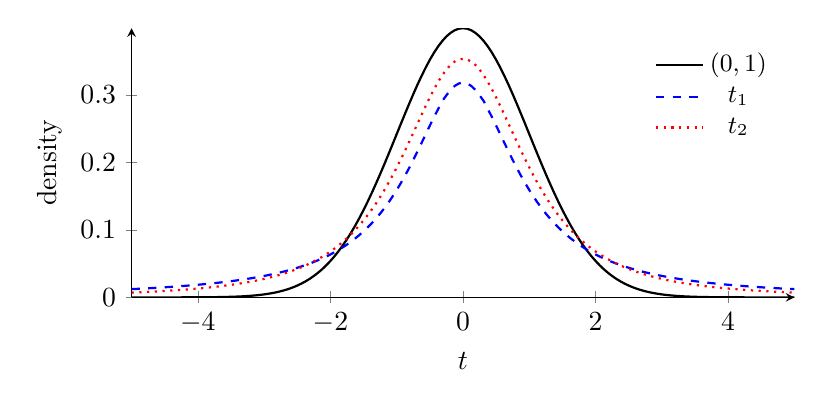
\begin{tikzpicture}
\begin{axis}[width=10cm,height=5cm,domain=-5:5,samples=161,axis lines=left,xlabel={$t$},ylabel={density},
  legend style={font=\small,draw=none,at={(0.98,0.95)},anchor=north east}]
\addplot[thick,black] {exp(-x^2/2)/sqrt(2*pi)};
\addplot[thick,blue,dashed] {1/(pi*(1+x^2))};
\addplot[thick,red,dotted] {0.3536*(1+x^2/2)^(-1.5)};
\legend{{$\N(0,1)$},{$t_1$},{$t_2$}}
\end{axis}
\end{tikzpicture}
\caption{The $t$ densities have heavier tails than the normal. This is why the critical values exceed $1.96$ when the degrees of freedom are small.}
\label{fig:L16-t}
\end{figure}

\subsection{Computation}
\begin{center}\small
\begin{tabular}{@{}>{\raggedright\arraybackslash}p{6.5cm}>{\raggedright\arraybackslash}p{8.9cm}@{}}\hline
R & Python\\\hline
\texttt{summary(lm.fit)} & \texttt{fit.summary()} (or \texttt{fit.params}, \texttt{fit.bse}, \texttt{fit.tvalues}, \texttt{fit.pvalues})\\
\texttt{confint(lm.fit)} & \texttt{fit.conf\_int()}\\
\texttt{pt(q, df)}, \texttt{qt(p, df)} & \texttt{scipy.stats.t.cdf(q, df)}, \texttt{stats.t.ppf(p, df)}\\
\texttt{pt(t, df, ncp)} & \texttt{stats.nct.cdf(t, df, ncp)}\\\hline
\end{tabular}
\end{center}
\nb{week05/L16\_intervals\_tests.ipynb} computes the coefficient table from the formulas, checks it against
\texttt{statsmodels}, and verifies the $95\%$ coverage and the $t_{n-p}$ distribution by simulation.

\subsection{Summary}
\begin{itemize}
  \item $s^2=\RSS/(n-r)$ is unbiased for $\sigma^2$, because $\EE[\eps\T M\eps]=\sigma^2\tr M$.
  \item Under normality: $\hat\beta\sim\N(\beta,\sigma^2(X\T X)^{-1})$, $\RSS/\sigma^2\sim\chi^2_{n-p}$, and they are independent. So $(\hat\beta_j-\beta_j)/\widehat{\mathrm{SE}}\sim t_{n-p}$.
  \item CI: $\hat\beta_j\pm t_{n-p,1-\alpha/2}\widehat{\mathrm{SE}}$. Test of $\beta_j=0$: $t=\hat\beta_j/\widehat{\mathrm{SE}}$.
  \item Boston: $\hat\beta_1=-0.9500$ (SE $0.0387$), CI $(-1.0261,-0.8740)$.
\end{itemize}

\subsection{Exercises}
\begin{problem}\label{prob:L16-1}
For the snowfall data of \cref{ex:L07-snow}, test $H_0:\beta_1=0$ at the $5\%$ level and give a $95\%$ CI for the slope.
\end{problem}
\begin{problem}\label{prob:L16-2}
Show that in simple linear regression the $t$ statistic for $\beta_1=0$ can be written $t=r\sqrt{n-2}/\sqrt{1-r^2}$, where $r$ is the sample correlation.
\end{problem}
\begin{problem}\label{prob:L16-3}
Why can we not use $\RSS/n$ in place of $s^2$ in \cref{thm:L16-dist}(4)? What is $\EE[\RSS/n]$?
\end{problem}
\begin{problem}\label{prob:L16-4}
In \cref{ex:L16-hand}, test $H_0:\beta_1=1$ against $\beta_1\ne 1$ at the $5\%$ level.
\end{problem}
\begin{problem}\label{prob:L16-5}
Simulate $10\,000$ data sets from $Y_i=0.5+1.4x_i+\eps_i$, $\eps_i\sim\N(0,0.1)$, $x=(1,2,3,4)$, and estimate the coverage of the $95\%$ interval for $\beta_1$.
\end{problem}

\subsection{Further reading}
Christensen, \S2.6 (sampling distributions), Chapter~3 (testing) and Chapter~6; Rao, \S4b (tests of linear
hypotheses); ISLR \S3.1.2.

% ============================================================
% Lecture 17 -- Assess the linear model by RSE and R-square
% ============================================================
\section{Assessing the Linear Model: RSE and $R^2$}\label{sec:L17}

\lectureheader{17}{g1UzPzHITGs}{Week-5 R code \texttt{Feb21.r} (``discuss what each summary is stating''). The Week-5 lecture PDF was \emph{not} accessed. Definitions follow ISLR \S3.1.3, which the code follows.}

\begin{guiding*}
By the end of this lecture you should be able to:
\begin{itemize}
  \item define the residual standard error (RSE) and $R^2$ and interpret them;
  \item prove the decomposition $\TSS=\mathrm{ESS}+\RSS$ when the model contains an intercept;
  \item prove that $R^2=r^2$ in simple linear regression;
  \item read the bottom part of \texttt{summary(lm(...))}.
\end{itemize}
\end{guiding*}

\subsection{Recap}
\Cref{sec:L16} judged individual coefficients: is $\beta_j$ zero or not? Here we judge the fit of the model as a
whole: how far are the data from the fitted line, and how much of the variation in $Y$ does the model explain?

\subsection{Residual standard error}
\begin{definition}[Residual standard error]\label{def:L17-rse}
For a model with $\rank X=p$ fitted to $n$ observations,
\[
\RSE=\sqrt{\frac{\RSS}{n-p}}=s,\qquad \RSS=\sum_{i=1}^n(Y_i-\hat Y_i)^2 .
\]
In simple linear regression, $\RSE=\sqrt{\RSS/(n-2)}$.
\end{definition}
The RSE estimates $\sigma$, the standard deviation of the errors (\cref{thm:L16-s2}). It is roughly the
typical size of the amount by which a response deviates from the true regression line, measured in the
units of $Y$. It is an absolute measure of \emph{lack of fit}. Whether a given RSE is ``small'' depends on
the scale of $Y$.

\subsection{The coefficient of determination}
\begin{definition}[$R^2$]\label{def:L17-r2}
For a model containing an intercept ($\one_n\in\colsp{X}$), let $\TSS=\sum_i(Y_i-\bar Y)^2$ and
$\mathrm{ESS}=\sum_i(\hat Y_i-\bar Y)^2$ (the explained sum of squares). Then
\[
R^2=1-\frac{\RSS}{\TSS}=\frac{\mathrm{ESS}}{\TSS}.
\]
\end{definition}
The second equality is the following theorem.

\begin{theorem}[Decomposition of TSS]\label{thm:L17-decomp}
If $\one_n\in\colsp{X}$, then $\TSS=\mathrm{ESS}+\RSS$, and $0\le R^2\le 1$.
\end{theorem}
\begin{proof}
Write $Y-\bar Y\one=(\hat Y-\bar Y\one)+(Y-\hat Y)$. The second vector $\hat e=Y-\hat Y=(I-\PX)Y$ is orthogonal to
$\colsp{X}$. The first vector lies in $\colsp{X}$, since $\hat Y\in\colsp{X}$ and $\one\in\colsp{X}$. Hence the cross term
vanishes and, by Pythagoras,
$\pnorm{Y-\bar Y\one}^2=\pnorm{\hat Y-\bar Y\one}^2+\pnorm{\hat e}^2$, i.e.\ $\TSS=\mathrm{ESS}+\RSS$. Both parts are
non-negative, so $0\le\RSS/\TSS\le1$.
\end{proof}
This is the same decomposition as $\TSS=\SSB+\SSW$ in the one-way model (\cref{thm:L08-decomp}). There
$\hat Y_{ij}=\bar Y_{i\cdot}$, so $\mathrm{ESS}=\SSB$ and $\RSS=\SSW$.

$R^2$ is the \emph{proportion of the variability in $Y$ explained by the model}. It is a relative measure, always
between $0$ and $1$ and free of units. $R^2$ near $1$ means that the model explains most of the variation. $R^2$
near $0$ means that it explains little: either the linear model is wrong or the errors are large.

\begin{theorem}\label{thm:L17-r2r}
In simple linear regression, $R^2=r^2$, where $r=S_{xY}/\sqrt{S_{xx}S_{YY}}$ is the sample correlation.
\end{theorem}
\begin{proof}
By \cref{thm:L05-slr}, $\RSS=S_{YY}-S_{xY}^2/S_{xx}$ and $\TSS=S_{YY}$. So
$R^2=1-\RSS/\TSS=\dfrac{S_{xY}^2}{S_{xx}S_{YY}}=r^2$.
\end{proof}

\begin{example}[The four-point data]\label{ex:L17-hand}
$Y=(2,3,5,6)$, $\bar Y=4$, $\TSS=4+1+1+4=10$, and $\RSS=0.2$. So
$R^2=1-0.2/10=0.98$. Also $r=7/\sqrt{5\times10}=0.98995$ and $r^2=0.98$. \checkmark\ Fitted values
$(1.9,3.3,4.7,6.1)$ give $\mathrm{ESS}=2.1^2+0.7^2+0.7^2+2.1^2=9.8=\TSS-\RSS$. $\RSE=\sqrt{0.2/2}=0.3162$.
\end{example}

\begin{example}[Boston and iris]\label{ex:L17-boston}
For \texttt{lm(medv \textasciitilde\ lstat, data = Boston)}:
$\RSS=19472.38$, $\TSS=42716.30$, so $R^2=1-19472.38/42716.30=0.5441$, and
$\RSE=\sqrt{19472.38/504}=6.216$. \texttt{summary} prints: ``Residual standard error: 6.216 on 504 degrees of freedom,
Multiple R-squared: 0.5441, Adjusted R-squared: 0.5432, F-statistic: 601.6 on 1 and 504 DF''. So
\texttt{lstat} explains about $54\%$ of the variation in median house values, and a typical prediction is off by about
\$6200. Since $\bar{\texttt{medv}}=22.53$, that is a relative error of about $28\%$.
For \texttt{iris} (\cref{ex:L15-iris}): $R^2=0.6690$ and $\RSE=0.4780$ on $148$ degrees of freedom.
\end{example}

\begin{note}[Supplementary: adjusted $R^2$ and the $F$ statistic]
Adding columns to $X$ can never increase $\RSS$: minimising over a larger column space gives a smaller or equal
minimum. So $R^2$ always increases when variables are added, even useless ones. The \emph{adjusted}
$R^2_{\mathrm{adj}}=1-\frac{\RSS/(n-p)}{\TSS/(n-1)}$ penalises this. For Boston it is $1-\frac{19472.38/504}{42716.30/505}=0.5432$.
The $F$ statistic $\frac{\mathrm{ESS}/(p-1)}{\RSS/(n-p)}=\frac{23243.91/1}{19472.38/504}=601.6$ tests whether all slopes are
zero. With one predictor, $F=t^2=(-24.528)^2$. The $F$-test is the subject of Week~8.
\end{note}

\subsection{Computation}
\texttt{fit.rsquared}, \texttt{fit.rsquared\_adj}, \texttt{np.sqrt(fit.scale)} (RSE), \texttt{fit.ssr} (RSS),
\texttt{fit.centered\_tss} (TSS), \texttt{fit.ess}, \texttt{fit.fvalue}. See \nb{week05/L17\_rse\_rsquared.ipynb}, which
computes everything from the definitions and checks it against \texttt{statsmodels}. It also illustrates that
$R^2$ never decreases when a pure-noise variable is added, while $R^2_{\mathrm{adj}}$ can.

\subsection{Summary}
\begin{itemize}
  \item $\RSE=\sqrt{\RSS/(n-p)}$ estimates $\sigma$. It is an absolute measure of lack of fit, in the units of $Y$.
  \item With an intercept, $\TSS=\mathrm{ESS}+\RSS$ and $R^2=1-\RSS/\TSS\in[0,1]$ is the proportion of variance explained.
  \item Simple linear regression: $R^2=r^2$. Boston: $R^2=0.544$, $\RSE=6.216$.
\end{itemize}

\subsection{Exercises}
\begin{problem}\label{prob:L17-1}
Show by example that without an intercept, $1-\RSS/\TSS$ can be negative.
\end{problem}
\begin{problem}\label{prob:L17-2}
Show that $R^2$ equals the squared sample correlation between $Y_i$ and $\hat Y_i$ in any model with an intercept.
\end{problem}
\begin{problem}\label{prob:L17-3}
If $Y$ is measured in different units ($Y'=cY$, $c\ne0$), how do $\RSE$ and $R^2$ change?
\end{problem}
\begin{problem}\label{prob:L17-4}
Compute $R^2$ for the one-way example of \cref{ex:L08-SS} (groups $\{5,7\},\{8,10,12\},\{4,6\}$).
\end{problem}

\subsection{Further reading}
ISLR \S3.1.3 (assessing the accuracy of the model); Christensen, \S6.4 and Chapter~14 (coefficient of
determination); Weisberg, \emph{ALR}, \S2.7 and \S3.4.

% ============================================================
% Lecture 18 -- Computation of least square estimates in R
% ============================================================
\section{Computation of Least Squares Estimates in R}\label{sec:L18}

\lectureheader{18}{4gwbWg_Gq-4}{Week-5 R code \texttt{Feb21.r} (Boston lab: \texttt{names}, \texttt{coef}, \texttt{confint}, \texttt{predict}, diagnostic plots, \texttt{hatvalues}; Monte Carlo simulation; non-central $t$). The Week-5 lecture PDF was \emph{not} accessed.}

\begin{guiding*}
By the end of this lecture you should be able to:
\begin{itemize}
  \item extract every component of a fitted linear model in R and in Python;
  \item distinguish a confidence interval for the mean response from a prediction interval for a new response, and derive both;
  \item produce and interpret the four standard diagnostic plots;
  \item compute leverages (hat values) and identify high-leverage points;
  \item run a simple Monte Carlo simulation.
\end{itemize}
\end{guiding*}

\subsection{Recap}
The previous three lectures gave the estimates (\cref{sec:L15}), their standard errors, intervals and tests
(\cref{sec:L16}), and overall measures of fit (\cref{sec:L17}). This lecture walks through the rest of the R
code, which uses these results in practice on the \texttt{Boston} data.

\subsection{Inside a fitted model}
\texttt{names(lm.fit)} lists the stored components: \texttt{coefficients}, \texttt{residuals},
\texttt{fitted.values}, \texttt{rank}, \texttt{df.residual}, the QR decomposition, and others. \texttt{coef(lm.fit)} returns
$(34.5538,-0.9500)$ and \texttt{confint(lm.fit)} the intervals of \cref{ex:L16-boston}.

\begin{note}[How R actually solves the normal equations]
\texttt{lm} does not form $X\T X$. It computes a QR decomposition $X=QR$, where $Q$ ($n\times p$) has orthonormal columns
and $R$ ($p\times p$) is upper triangular. Then $X\T X\beta=X\T Y$ becomes $R\T R\beta=R\T Q\T Y$, i.e.\ $R\beta=Q\T Y$,
which is solved by back-substitution. This is numerically more stable, because the condition number of $X\T X$ is the
square of that of $X$. It also gives $\PX=QQ\T$ directly: $Q$ is an orthonormal basis of $\colsp{X}$, as in
\cref{lem:L14-projection}. \texttt{statsmodels} uses the Moore--Penrose pseudo-inverse by default, or QR with
\texttt{method="qr"}.
\end{note}

\subsection{Confidence and prediction intervals}
\texttt{predict(lm.fit, data.frame(lstat = c(5,10,15)), interval = "confidence")} and
\texttt{interval = "prediction"} give two different kinds of interval. At a new value $x_0$, let
$\hat Y_0=\hat\beta_0+\hat\beta_1x_0$ and $h_0=\frac1n+\frac{(x_0-\bar x)^2}{S_{xx}}$.

\begin{proposition}\label{prop:L18-intervals}
Assume normal errors in simple linear regression, and let $Y_0=\beta_0+\beta_1x_0+\eps_0$ be a new observation with
$\eps_0\sim\N(0,\sigma^2)$ independent of the data.
\begin{enumerate}
  \item $\hat Y_0\pm t_{n-2,1-\alpha/2}\,s\sqrt{h_0}$ is a $100(1-\alpha)\%$ \vocab{confidence interval} for the mean response $\beta_0+\beta_1x_0$.
  \item $\hat Y_0\pm t_{n-2,1-\alpha/2}\,s\sqrt{1+h_0}$ is a $100(1-\alpha)\%$ \vocab{prediction interval} for $Y_0$.
\end{enumerate}
\end{proposition}
\begin{proof}
$\hat Y_0=\lambda\T\hat\beta$ with $\lambda=(1,x_0)\T$. It is normal with mean $\beta_0+\beta_1x_0$ and variance
$\sigma^2\lambda\T(X\T X)^{-1}\lambda=\sigma^2h_0$ (\cref{prob:L15-3}). It is independent of $s^2$ (\cref{thm:L16-dist}).
(1) Then $(\hat Y_0-\beta_0-\beta_1x_0)/(s\sqrt{h_0})\sim t_{n-2}$, exactly as in the proof of \cref{thm:L16-dist}(4).
(2) $Y_0-\hat Y_0$ has mean $0$ and, since $\eps_0$ is independent of $\hat Y_0$, variance $\sigma^2+\sigma^2h_0$. It is
normal, and it is independent of $s^2$, because $\eps_0$ is independent of all the data. Hence
$(Y_0-\hat Y_0)/(s\sqrt{1+h_0})\sim t_{n-2}$, and the interval follows as in \cref{cor:L16-ci}.
\end{proof}
The confidence interval reflects only the uncertainty in the fitted line. It shrinks to zero width as
$n\to\infty$. The prediction interval also contains the irreducible noise $\eps_0$ of a new observation, so it never
becomes narrower than about $\pm1.96\sigma$.

\begin{example}[Boston]\label{ex:L18-predict}
With $n=506$, $s=6.2158$ and $t_{504,0.975}=1.9647$:
\begin{center}
\begin{tabular}{cccc}\hline
\texttt{lstat} & fit & 95\% confidence interval & 95\% prediction interval\\\hline
5 & 29.8036 & (29.0074, 30.5998) & (17.5657, 42.0415)\\
10 & 25.0533 & (24.4741, 25.6326) & (12.8276, 37.2791)\\
15 & 20.3031 & (19.7316, 20.8746) & (8.0777, 32.5285)\\\hline
\end{tabular}
\end{center}
Both intervals are centred at the same fitted value. The prediction intervals are about $20$ times wider.
\end{example}

\begin{example}[By hand]\label{ex:L18-hand}
For the four-point data at $x_0=5$: $\hat Y_0=0.5+1.4\times5=7.5$ and
$h_0=\frac14+\frac{(5-2.5)^2}{5}=1.5$ (an extrapolation, so $h_0$ is large). With $s^2=0.1$ and $t_{2,0.975}=4.3027$:
the confidence interval is $7.5\pm4.3027\sqrt{0.15}=7.5\pm1.6664=(5.8336,\,9.1664)$, and the prediction interval is
$7.5\pm4.3027\sqrt{0.25}=7.5\pm2.1514=(5.3487,\,9.6514)$.
\end{example}

\subsection{Diagnostic plots and leverage}
\texttt{par(mfrow=c(2,2)); plot(lm.fit)} draws four diagnostic plots: residuals against fitted values, a normal
Q--Q plot, a scale--location plot, and residuals against leverage. The code then draws
\texttt{plot(predict(lm.fit), residuals(lm.fit))} and \texttt{plot(predict(lm.fit), rstudent(lm.fit))}.
For Boston, the residuals against fitted values form a clear U-shape (\cref{fig:L18-diag}). This is evidence of
\emph{non-linearity}, exactly as in Forbes' data (\cref{sec:L06}). ISLR's lab later adds a term
$\texttt{lstat}^2$.

\begin{definition}[Leverage]\label{def:L18-leverage}
The \vocab{leverage} (hat value) of observation $i$ is $h_{ii}=(\PX)_{ii}$, the $i$th diagonal entry of the hat matrix.
The name comes from $\hat Y=\PX Y$: the projection matrix ``puts the hat on $Y$''. The
\vocab{studentized residual} (R: \texttt{rstudent}) is $\hat e_i/(s_{(i)}\sqrt{1-h_{ii}})$, where $s_{(i)}$ is the RSE of
the fit without observation $i$.
\end{definition}

\begin{proposition}\label{prop:L18-hat}
(1) $0\le h_{ii}\le1$ and $\sum_ih_{ii}=\rank X$. (2) $\Var(\hat e_i)=\sigma^2(1-h_{ii})$. (3) In simple linear regression
$h_{ii}=\frac1n+\frac{(x_i-\bar x)^2}{S_{xx}}$.
\end{proposition}
\begin{proof}
(1) Since $\PX$ is symmetric and idempotent, $h_{ii}=(\PX^2)_{ii}=\sum_l(\PX)_{il}^2=h_{ii}^2+\sum_{l\ne i}(\PX)_{il}^2\ge h_{ii}^2$. So
$h_{ii}\ge h_{ii}^2$, which gives $0\le h_{ii}\le1$. Also $\sum_ih_{ii}=\tr\PX=\rank X$ (\cref{lem:L14-projection}).
(2) $\hat e=(I-\PX)Y$, so $\Cov(\hat e)=\sigma^2(I-\PX)(I-\PX)\T=\sigma^2(I-\PX)$. Its $i$th diagonal entry is $\sigma^2(1-h_{ii})$.
(3) $h_{ii}=x_i\T(X\T X)^{-1}x_i$ with $x_i=(1,x_i)\T$. Using the inverse in the proof of \cref{cor:L15-slr},
$h_{ii}=\frac{\sum_lx_l^2-2x_i\sum_lx_l+nx_i^2}{nS_{xx}}=\frac{S_{xx}+n(x_i-\bar x)^2}{nS_{xx}}$. This is the stated formula, since
$\sum_lx_l^2-2x_i n\bar x+nx_i^2=S_{xx}+n\bar x^2-2nx_i\bar x+nx_i^2$.
\end{proof}
A point with large leverage has an $x$-value far from $\bar x$. It can pull the fitted line towards itself. For Boston,
\texttt{which.max(hatvalues(lm.fit))} returns observation $375$, which has the largest \texttt{lstat} ($37.97$) and
$h_{375,375}=0.02687$. The average leverage is $p/n=2/506=0.00395$, and the hat values sum to exactly $2$.

\begin{figure}[ht]
\centering
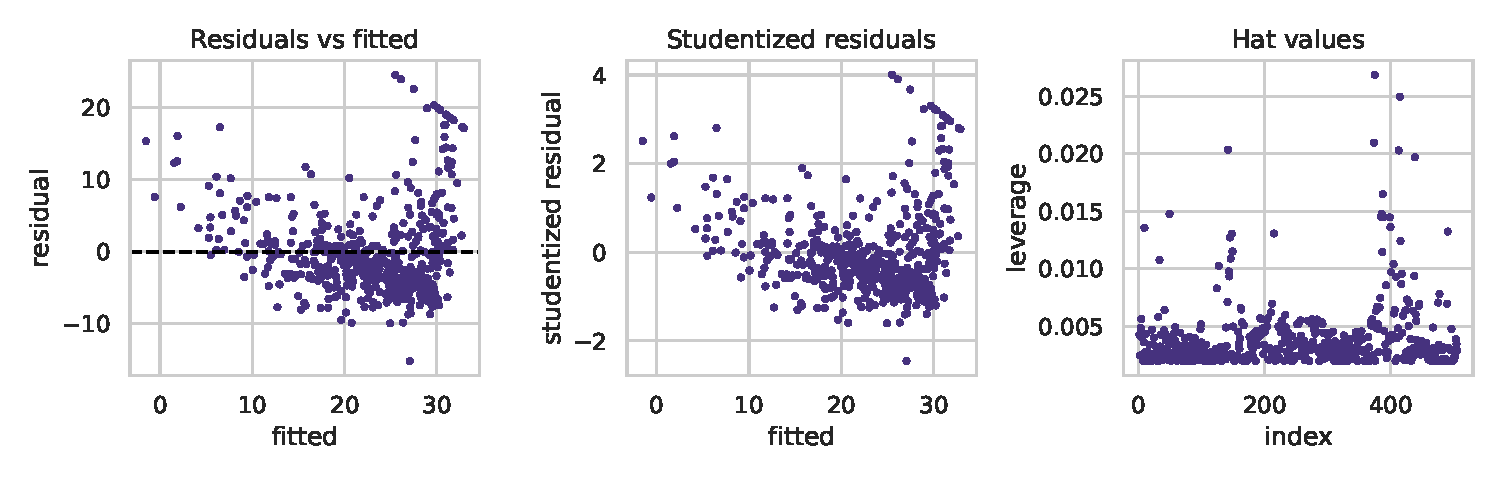
\includegraphics[width=\textwidth]{figures/L18_boston_diag.pdf}
\caption{Boston: residuals and studentized residuals against fitted values (note the curvature), and hat values
by observation index (the maximum is at observation 375).}
\label{fig:L18-diag}
\end{figure}

\subsection{A Monte Carlo simulation}
The code ends with a simulation:
\begin{center}
\begin{minipage}{0.8\textwidth}\small\ttfamily
OneFourthPiSamples = replicate(100, \{ u <- runif(10000); v <- runif(10000);\\
\quad z <- sqrt(u\textasciicircum2 + v\textasciicircum2); sum(z < 1)/10000 \})
\end{minipage}
\end{center}
A point $(U,V)$ uniform on the unit square falls inside the quarter disc $\{u^2+v^2<1\}$ with probability equal to its area,
$\pi/4=0.7854$. Each replicate estimates $\pi/4$ by the proportion of $10\,000$ points inside, with standard error
$\sqrt{(\pi/4)(1-\pi/4)/10000}=0.0041$. With the notebook's seed the $100$ replicates have mean $0.7858$ and
standard deviation $0.0047$. The same idea, repeat an experiment and look at the distribution of an estimate, is how the
notebooks check sampling distributions such as those of \cref{thm:L16-dist}. The instructor uses it for least squares
estimators in Week~7.

\subsection{Computation}
\begin{center}\small
\begin{tabular}{@{}>{\raggedright\arraybackslash}p{7cm}>{\raggedright\arraybackslash}p{8.4cm}@{}}\hline
R & Python (\texttt{statsmodels})\\\hline
\texttt{names(lm.fit)}, \texttt{coef}, \texttt{confint} & \texttt{dir(fit)}, \texttt{fit.params}, \texttt{fit.conf\_int()}\\
\texttt{predict(..., interval="confidence")} & \texttt{fit.get\_prediction(new).summary\_frame()} (\texttt{mean\_ci\_*})\\
\texttt{predict(..., interval="prediction")} & same frame, columns \texttt{obs\_ci\_*}\\
\texttt{plot(lm.fit)} & residual, Q--Q (\texttt{sm.qqplot}), leverage plots\\
\texttt{hatvalues}, \texttt{rstudent} & \texttt{fit.get\_influence().hat\_matrix\_diag}, \texttt{.resid\_studentized\_external}\\
\texttt{replicate(100, \{...\})} & list comprehension with \texttt{rng.uniform}\\\hline
\end{tabular}
\end{center}
See \nb{week05/L18\_computation\_in\_R.ipynb}.

\subsection{Summary}
\begin{itemize}
  \item At $x_0$: confidence interval $\hat Y_0\pm t\,s\sqrt{h_0}$ for the mean, prediction interval $\hat Y_0\pm t\,s\sqrt{1+h_0}$ for a new $Y$, where $h_0=\frac1n+\frac{(x_0-\bar x)^2}{S_{xx}}$.
  \item Leverage $h_{ii}=(\PX)_{ii}\in[0,1]$, $\sum h_{ii}=p$, $\Var\hat e_i=\sigma^2(1-h_{ii})$.
  \item Boston: the residuals show curvature, and the highest leverage is observation $375$.
  \item Monte Carlo: repeat, then summarise the estimates.
\end{itemize}

\subsection{Exercises}
\begin{problem}\label{prob:L18-1}
Show that the prediction interval at $x_0=\bar x$ has half-width $t_{n-2,1-\alpha/2}\,s\sqrt{1+1/n}$.
\end{problem}
\begin{problem}\label{prob:L18-2}
For the four-point data compute all four hat values and check that they sum to $2$.
\end{problem}
\begin{problem}\label{prob:L18-3}
Fit \texttt{medv \textasciitilde\ lstat + I(lstat\textasciicircum2)} and compare $R^2$ and the residual plot with the straight-line fit.
\end{problem}
\begin{problem}\label{prob:L18-4}
Estimate $\pi$ by Monte Carlo with $10^6$ points. How many points are needed for the standard error of the estimate of $\pi$ to be below $0.001$?
\end{problem}

\subsection{Further reading}
ISLR \S3.1--3.3 and Lab~3.6; Weisberg, \emph{ALR}, Chapter~9 (regression diagnostics); Christensen, Chapter~12.


\section*{Solutions to the Exercises of Chapter~\ref{ch:week05}}
\addcontentsline{toc}{section}{Solutions to the exercises}

\paragraph{\Cref{prob:L15-1}.}
Since $\sum_i(x_i-\bar x)=0$, $S_{xy}=\sum_i(x_i-\bar x)(Y_i-\bar Y)=\sum_i(x_i-\bar x)Y_i$. So
$\hat\beta_1=S_{xy}/S_{xx}=\sum_ic_iY_i$. Then $\sum_ic_i=\sum_i(x_i-\bar x)/S_{xx}=0$, and
$\sum_ic_ix_i=\sum_i(x_i-\bar x)x_i/S_{xx}=\sum_i(x_i-\bar x)^2/S_{xx}=1$, again because $\sum_i(x_i-\bar x)\bar x=0$.
It follows that $\EE\hat\beta_1=\sum_ic_i(\beta_0+\beta_1x_i)=\beta_1$ and $\Var\hat\beta_1=\sigma^2\sum_ic_i^2=\sigma^2/S_{xx}$.

\paragraph{\Cref{prob:L15-2}.}
$X\T X=\begin{pmatrix}3&\sum x_i\\\sum x_i&\sum x_i^2\end{pmatrix}=\begin{pmatrix}3&0\\0&2\end{pmatrix}$, so
$\Cov(\hat\beta)=\sigma^2(X\T X)^{-1}=\sigma^2\operatorname{diag}(1/3,\,1/2)$. By \cref{cor:L15-slr},
$\Cov(\hat\beta_0,\hat\beta_1)=-\sigma^2\bar x/S_{xx}$, which is $0$ because the design is centred ($\bar x=0$). Then
$\hat\beta_0=\bar Y$ and $\hat\beta_1$ is a contrast of the $Y_i$, orthogonal to $\one$.

\paragraph{\Cref{prob:L15-3}.}
Write $\hat\beta_0+\hat\beta_1x_0=\bar Y+\hat\beta_1(x_0-\bar x)$. Now
$\Cov(\bar Y,\hat\beta_1)=\sum_i\frac1n c_i\sigma^2=0$ by \cref{prob:L15-1}. Hence
$\Var=\frac{\sigma^2}n+(x_0-\bar x)^2\frac{\sigma^2}{S_{xx}}$. (Equivalently, $\sigma^2 x_0\T(X\T X)^{-1}x_0$ with $x_0=(1,x_0)\T$.)

\paragraph{\Cref{prob:L15-4}.}
$\Var\hat\beta_1=\sigma^2/S_{xx}$, so we maximise $S_{xx}$. For $x_i\in[0,1]$, $x_i^2\le x_i$, so
$S_{xx}=\sum x_i^2-n\bar x^2\le n\bar x-n\bar x^2=n\bar x(1-\bar x)\le n/4$. Equality needs every $x_i\in\{0,1\}$ and
$\bar x=1/2$: put five points at $0$ and five at $1$, giving $S_{xx}=2.5$. Ten equally spaced points give only $S_{xx}=1.019$.
(This design is optimal only if the model is known to be linear. With two support points we cannot check linearity.)

\paragraph{\Cref{prob:L16-1}.}
For the Fort Collins data ($n=93$): $\hat\beta_1=0.2035$, $\widehat{\mathrm{SE}}=0.1310$, $t=1.553$ on $91$ degrees of freedom,
$p=0.124>0.05$. We do not reject $H_0:\beta_1=0$. The $95\%$ CI is $0.2035\pm1.9864\times0.1310=(-0.0568,\,0.4638)$, which
contains $0$. Early-season snowfall tells us little about late-season snowfall.

\paragraph{\Cref{prob:L16-2}.}
$\hat\beta_1=S_{xy}/S_{xx}=r\sqrt{S_{yy}/S_{xx}}$ and $\RSS=S_{yy}-S_{xy}^2/S_{xx}=S_{yy}(1-r^2)$. So
$s^2=S_{yy}(1-r^2)/(n-2)$, and
\[
t=\frac{\hat\beta_1}{s/\sqrt{S_{xx}}}=\frac{r\sqrt{S_{yy}/S_{xx}}\sqrt{S_{xx}}\sqrt{n-2}}{\sqrt{S_{yy}(1-r^2)}}=\frac{r\sqrt{n-2}}{\sqrt{1-r^2}}.
\]
For the snowfall data this gives $1.5528$, the same as the regression $t$.

\paragraph{\Cref{prob:L16-3}.}
The $t$ pivot uses the fact that $(n-p)s^2/\sigma^2=\RSS/\sigma^2\sim\chi^2_{n-p}$, independent of $\hat\beta$. A $t_{n-p}$ variable is
$Z/\sqrt{\chi^2_{n-p}/(n-p)}$, so the divisor must be $n-p$. With $\RSS/n$ the ratio is $\sqrt{n/(n-p)}\,T$, not $t_{n-p}$. It is
also biased: $\EE[\RSS/n]=\frac{n-p}{n}\sigma^2<\sigma^2$ (\cref{thm:L16-s2}). Intervals built from it would be too short.

\paragraph{\Cref{prob:L16-4}.}
$t=(1.4-1)/0.14142=2.828<t_{2,0.975}=4.303$ (two-sided $p=0.106$). We do not reject $\beta_1=1$. This agrees with
$1\in(0.7915,\,2.0085)$ from \cref{ex:L16-hand}.

\paragraph{\Cref{prob:L16-5}.}
With $\sigma^2=0.1$ and $10\,000$ replicates, the notebook finds coverage $0.9499$, within Monte Carlo error
($\pm0.0044$) of $0.95$. The interval is exact for normal errors, whatever $\sigma^2$ and $n$ are.

\paragraph{\Cref{prob:L17-1}.}
Take $x=(1,2,3)$, $y=(3,2,1)$ and fit $y=\beta x$ through the origin. Then $\hat\beta=\sum x_iy_i/\sum x_i^2=10/14=5/7$, the
residuals are $(16,4,-8)/7$, $\RSS=48/7\approx6.857$, and the centred $\TSS=2$. So $1-\RSS/\TSS=-17/7\approx-2.43$.
Without an intercept, $\one\notin\colsp{X}$, the decomposition $\TSS=\mathrm{ESS}+\RSS$ fails, and a line through the
origin can do worse than the constant $\bar y$.

\paragraph{\Cref{prob:L17-2}.}
With an intercept, $\one\in\colsp{X}$, so $\sum_ie_i=0$ and the mean of the $\hat Y_i$ is $\bar Y$. Since $e\perp\hat Y-\bar Y\one$,
\[
\sum_i(Y_i-\bar Y)(\hat Y_i-\bar Y)=\sum_i(\hat Y_i-\bar Y+e_i)(\hat Y_i-\bar Y)=\mathrm{ESS}.
\]
Hence $\operatorname{corr}(Y,\hat Y)^2=\mathrm{ESS}^2/(\TSS\cdot\mathrm{ESS})=\mathrm{ESS}/\TSS=R^2$ by \cref{thm:L17-decomp}.

\paragraph{\Cref{prob:L17-3}.}
$\hat\beta'=c\hat\beta$ and $e'=ce$, so $\RSS'=c^2\RSS$ and $\TSS'=c^2\TSS$. Thus $\RSE'=\abs c\,\RSE$ (RSE is in the units of $Y$),
while $R^2$ is unchanged (it is unit-free).

\paragraph{\Cref{prob:L17-4}.}
The one-way model contains the intercept (as the sum of the group indicators), so $\RSS=\SSW=12=84/7$ and
$\TSS=\SSW+\SSB=84/7+250/7=334/7$. Hence $R^2=\SSB/\TSS=250/334=125/167\approx0.7485$.

\paragraph{\Cref{prob:L18-1}.}
By \cref{prop:L18-intervals} the prediction half-width is $t_{n-2,1-\alpha/2}\,s\sqrt{1+h_0}$ with
$h_0=\frac1n+\frac{(x_0-\bar x)^2}{S_{xx}}$. At $x_0=\bar x$, $h_0=1/n$. This is the narrowest prediction interval.

\paragraph{\Cref{prob:L18-2}.}
$h_i=\frac14+\frac{(x_i-2.5)^2}{5}$ gives $(0.7,0.3,0.3,0.7)$, the diagonal of $\PX$ in \cref{prob:L14-2}. The sum is
$2=\tr\PX=\rank X$ (\cref{prop:L18-hat}).

\paragraph{\Cref{prob:L18-3}.}
The quadratic fit is $\widehat{\texttt{medv}}=42.862-2.3328\,\texttt{lstat}+0.04355\,\texttt{lstat}^2$, with all terms highly
significant. $R^2$ rises from $0.5441$ to $0.6407$ and RSE falls from $6.216$ to $5.524$. The U-shape in the
residual-versus-fitted plot largely disappears, which confirms the non-linearity seen in \cref{fig:L18-diag}.

\paragraph{\Cref{prob:L18-4}.}
$\hat\pi=4\hat p$, where $\hat p$ is the fraction of $m$ uniform points inside the quarter disc. So
$\mathrm{SE}(\hat\pi)=4\sqrt{p(1-p)/m}$ with $p=\pi/4$. For $m=10^6$ this is $0.00164$ (the notebook's estimate is $3.14013$).
The condition $\mathrm{SE}<0.001$ requires $m>16p(1-p)/10^{-6}\approx2.70\times10^6$. Each extra decimal digit costs a factor of $100$ in
sample size.
